\section{Data understanding and preparation}\label{sec:m1}

\subsection{Data semantics}\label{sec:sem}
The dataset has 13\,843 rows and 33 columns. Each row is one seller (\attr{sp\_id}); every other column aggregates the listings observed for that seller. \Cref{tab:num} introduces the 24 numerical attributes together with their statistics and \cref{tab:cat} the categorical ones. The target \attr{seller\_rating\_class} is ordinal (\emph{low} $<$ \emph{medium} $<$ \emph{high}); the remaining categorical attributes are nominal. The documentation does not state units: those in \cref{tab:num} are inferred from the value ranges. \attr{sp\_id} is stored as a float but has no fractional part and no repetition, so it was cast to an integer and used only as an index.

Two consequences of the aggregation matter for the whole report. First, each numerical attribute is a \emph{median} over an inventory, so relations that hold car by car need not hold between columns (e.g.\ year $+$ age is not constant). Second, a seller with 5 listings and one with 4\,959 have the same weight, although the medians of the former are far noisier.

\begin{table*}[t]
\centering
\caption{Numerical attributes after cleaning: semantics, statistics, association with the target ($\eps^2$, Kruskal--Wallis effect size) and role in modelling (\emph{log1p}/\emph{raw}: scale used by distance-based and Gaussian methods; \emph{dropped}: eliminated in \cref{sec:corr}). Suffix \attr{\_median} omitted.}\label{tab:num}
\tabtight{m1_numeric}
\end{table*}

\begin{table}[t]
\centering
\caption{Categorical attributes: levels in the raw data, mode, missing values and treatment.}\label{tab:cat}
{\tabfont\setlength{\tabcolsep}{2.5pt}
\begin{tabular}{@{}l r l p{0.35\linewidth}@{}}
\toprule
Attribute & Lev. & Mode (\%) & Missing / treatment\\
\midrule
body\_type & 9 & SUV (64.4) & rare levels merged: 6 groups\\
fuel\_type & 7 & gasoline (98.7) & 1 \emph{unknown} $\to$ NaN; 4 groups\\
transmission & 4 & automatic (93.7) & 6 \emph{unknown} $\to$ NaN\\
wheel\_system & 5 & -- (NaN 76.0) & dropped\\
listing\_color & 11 & white (37.3) & 10.9\% \emph{unknown} kept as level; 8 groups\\
franchise\_status & 2 & franchise (50.6) & none\\
new\_used\_profile & 3 & used only (53.3) & none; function of \attr{pct\_is\_new}\\
rating\_class & 3 & medium (54.7) & target\\
\bottomrule
\end{tabular}}
\end{table}

\subsection{Distributions and statistics}
\paragraph{Target} The classes are imbalanced (\cref{fig:target}, left): 54.7\% \emph{medium}, 26.6\% \emph{high}, 18.6\% \emph{low}. A majority predictor already scores 0.547 accuracy, so \cref{sec:m3} uses stratified splits and selects models by macro-F1. The dealer type shifts the mix (\cref{fig:target}, right): independents are rated \emph{high} more often than franchises (33\% vs 21\%) and \emph{low} less often (16\% vs 21\%). The association is significant ($\chi^2=270$, $p<10^{-58}$) but weak (Cram\'er's $V=0.14$).

\begin{figure*}[t]
\centering
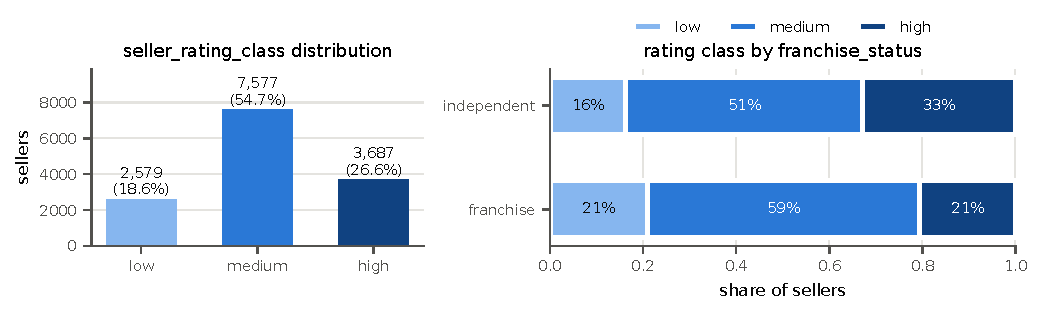
\includegraphics[width=0.92\textwidth]{m1_target_balance}
\caption{Class balance of the target (left) and rating mix by dealer type (right).}\label{fig:target}
\end{figure*}

\paragraph{Numerical attributes} Three shapes dominate \cref{tab:num,fig:log}. Volumes, prices and times are strongly right-skewed (\attr{daysonmarket} 8.8, \attr{city\_fuel\_economy} 8.1, \attr{n\_listings} 5.2). Inventory-mix shares are zero-inflated: 91\% of the sellers have no salvage vehicle, 85\% no theft title. \attr{pct\_is\_new} and \attr{mileage} are bimodal: 53\% of the sellers list no new car, while the rest form a new-car mode at almost zero mileage. This used/new duality is the main structure of the data and reappears in every module.

\begin{figure*}[t]
\centering
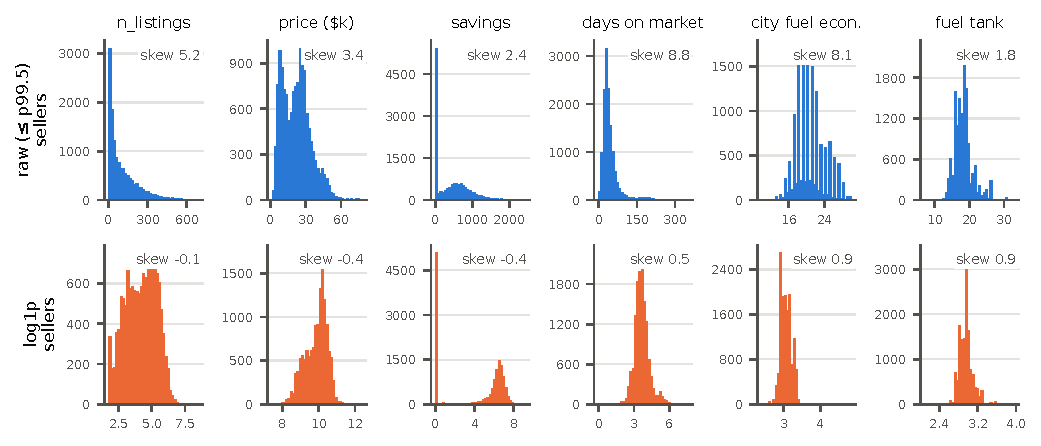
\includegraphics[width=0.97\textwidth]{m1_log_transform}
\caption{Log-transformed modelling attributes, raw scale clipped at $p_{99.5}$ (top) and \code{log1p} scale (bottom). \attr{savings\_amount} keeps its spike at zero: 37\% of the sellers advertise no savings.}\label{fig:log}
\end{figure*}

\begin{figure*}[t]
\centering
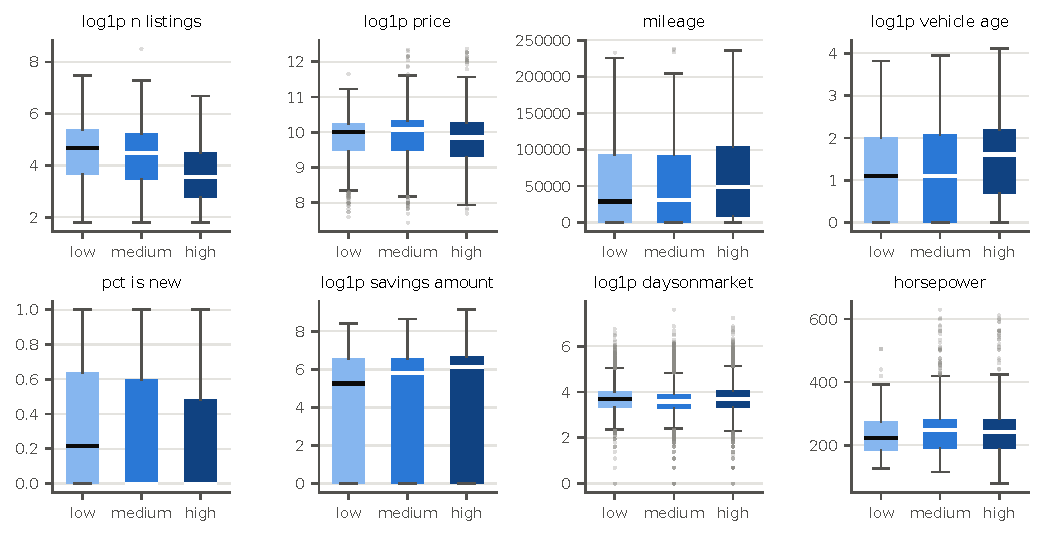
\includegraphics[width=0.97\textwidth]{m1_box_by_target}
\caption{Key attributes by rating class. Only seller size (\attr{n\_listings}) separates the classes visibly, and mainly \emph{high} from the other two.}\label{fig:box}
\end{figure*}

\paragraph{Attributes vs target} We used Kruskal--Wallis tests because of the skew. With 13\,843 sellers every attribute except \attr{front\_legroom} ($p=0.07$) is significant, so we read effect sizes instead of $p$-values ($\eps^2$ in \cref{tab:num}). Seller size is the only attribute with a moderate effect (\attr{n\_listings} $\eps^2=0.082$, \attr{n\_listing\_days} 0.073); all others are at most 0.017. Median size drops from 107 (\emph{low}) and 88 (\emph{medium}) to 34 listings for \emph{high} (\cref{fig:box}). High-rated sellers are typically small, used-car, independent dealers; \emph{low} and \emph{medium} overlap almost completely. This sets modest expectations for \cref{sec:m3}.

\paragraph{Categorical attributes} Most levels are very concentrated (\cref{fig:cat}): \attr{fuel\_type} and \attr{transmission} are almost constant, body type is dominated by SUVs, and colour by white and black. Only 31 sellers (0.2\%) sell new cars only. \attr{franchise\_status} shows just two of the four documented levels (\emph{mixed} and \emph{unknown} never occur).

\begin{figure*}[t]
\centering
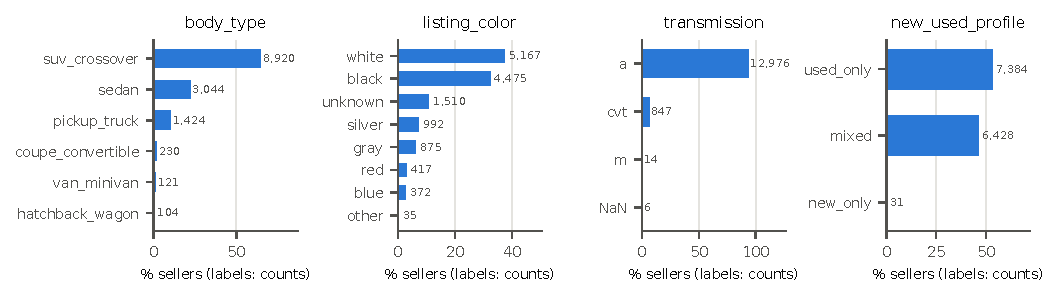
\includegraphics[width=0.97\textwidth]{m1_categorical}
\caption{Categorical attributes after the grouping of rare levels (labels: number of sellers).}\label{fig:cat}
\end{figure*}

\subsection{Data quality}\label{sec:quality}
\paragraph{Duplicates} There are no duplicate rows, no duplicate \attr{sp\_id}, and no two sellers with identical attributes.

\paragraph{Missing values} We looked for explicit \code{NaN} and for implicit codes (\emph{unknown}, empty strings, impossible zeros). Zeros are legitimate for savings, mileage, age, days on market, span and shares. Three attributes have relevant missingness (\cref{fig:miss}); all others are below 0.3\%. We tested whether missingness depends on the target or dealer type, because that decides between dropping and imputing:
\begin{itemize}
\item \attr{wheel\_system} (76.0\%): independent of the target ($\chi^2$ $p=0.32$) and of dealer type ($p=0.17$). Imputing it would invent three quarters of the column, so it was \textbf{dropped}.
\item \attr{engine\_displacement} (24.5\%): also independent of target ($p=0.21$) and dealer ($p=0.61$); \textbf{excluded} from modelling because of its missing rate and redundancy (\cref{sec:corr}).
\item \attr{listing\_color} = \emph{unknown} (10.9\%): 15.9\% for franchises but 5.8\% for independents ($p<10^{-80}$). The absence is informative, so it was \textbf{kept as a level}.
\end{itemize}
The 27 missing \attr{pct\_isCab}, \attr{pct\_salvage} and \attr{pct\_theft\_title} occur in the same rows, all (almost) new-only sellers. This missingness is structural (a new car cannot be an ex-taxi or a salvage), so they were set to 0 by rule.

The remaining \code{NaN}s are \emph{not} imputed here. Imputing on the whole dataset would leak test information into \cref{sec:m3}: medians and modes are fitted on all data only for the unsupervised analyses, and inside the training folds for supervised ones.

\begin{figure}[t]
\centering
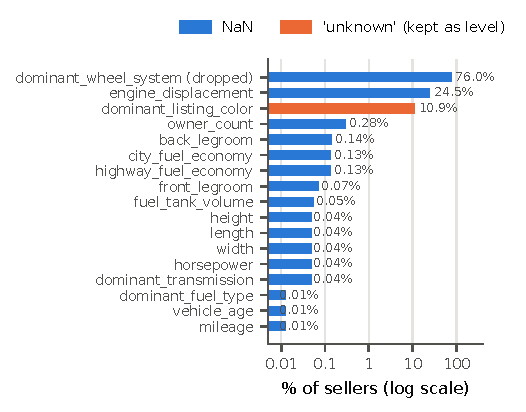
\includegraphics[width=0.92\linewidth]{m1_missing}
\caption{Missing values per attribute (log scale).}\label{fig:miss}
\end{figure}

\paragraph{Consistency checks} We evaluated 14 rules (\cref{tab:checks}). Only two reveal errors, and both were set to \code{NaN}; the others have a domain explanation that we checked on the records. For example, the 338 majority-new sellers with mileage above 5\,000 have a median vehicle age of 0: \attr{is\_new} marks recent model years, not zero-kilometre cars.

\begin{table}[t]
\centering
\caption{Consistency rules. No violation was found for negative values, shares outside $[0,1]$, \attr{new\_used\_profile} vs \attr{pct\_is\_new}, listing days vs listings/span, and savings $>$ price.}\label{tab:checks}
{\tabfont\setlength{\tabcolsep}{3pt}
\begin{tabular}{@{}p{0.43\linewidth}r p{0.41\linewidth}@{}}
\toprule
Rule violated & $n$ & Decision\\
\midrule
front legroom $>46$ in & 2 & error $\to$ NaN (54 and 67 in on SUVs)\\
non-electric economy $>60$ MPG & 2 & error $\to$ NaN (petrol, 210--388 hp)\\
\midrule
electric economy $>60$ & 8 & kept: MPGe unit\\
highway $<$ city economy & 18 & kept: hybrids, mixed stock\\
rear legroom $=0$ & 3 & kept: two-seat pickups, vans\\
model year $<1995$ & 38 & kept: classic-car dealers\\
year $+$ age $\notin[2018,2022]$ & 42 & kept: medians not additive\\
share new $>0.5$, mileage $>5$k & 338 & kept: recent model years\\
days on market $>$ span & 120 & kept: listed before window\\
\bottomrule
\end{tabular}}
\end{table}

\paragraph{Outliers} The $1.5\,$IQR rule on the modelling scale flags between 0\% and 6.7\% of the values of the continuous attributes (\attr{length} 6.7\%, \attr{daysonmarket} 6.1\%, \attr{fuel\_tank} 4.8\%). It is meaningless for zero-inflated shares, where $\mathrm{IQR}=0$ flags every non-zero value (15\% for \attr{pct\_theft\_title}). The extremes we inspected are real sellers: supercar dealers (up to \$236k), classic-car dealers (median \$34.9k vs \$22.3k), a 4\,959-listing dealer, heavy-duty trucks. We therefore \textbf{kept} all of them and limited their influence through log scales. Multivariate anomalies are analysed as DBSCAN noise (\cref{sec:dbscan}), and the effect of keeping them is measured in \cref{sec:m2core,sec:ablation}.

\subsection{Variable transformations}\label{sec:trans}
We applied \code{log1p} when the raw skewness exceeds 1 \emph{and} the log at least halves it; otherwise the transform only costs interpretability. This selects nine attributes (\attr{n\_listings}, \attr{price}, \attr{savings}, \attr{daysonmarket}, both fuel economies, \attr{fuel\_tank}, \attr{engine\_displacement}, \attr{vehicle\_age}) and rejects e.g.\ \attr{listing\_span} (2.15 $\to$ $-1.22$, over-corrected) and \attr{mileage} (bimodal, $0.68\to-0.91$). Rare categorical levels ($<1\%$) were merged by meaning (e.g.\ coupe $+$ convertible), because they produce unstable splits and itemsets.

Each task uses its own view of the same clean base: log $+$ standardized for distances and Gaussians (K-Means, DBSCAN, KNN, GaussianNB), raw for trees (invariant to monotone transforms), binned for CategoricalNB and pattern mining. Whether these choices matter is tested by ablation in \cref{sec:m2attr,sec:ablation}.

\subsection{Pairwise correlations and elimination}\label{sec:corr}
Spearman's $\rho_s$ is the main criterion, since relations are monotone but not linear (price--mileage: $r=-0.68$, $\rho_s=-0.82$). \Cref{fig:heat} shows two blocks: \emph{newness} (mileage, year, age, owners, share of new, price) and \emph{vehicle size and power} (horsepower, displacement, tank, dimensions, and inversely fuel economy). \Cref{tab:corr} lists the strongest pairs.

\begin{figure*}[t]
\centering
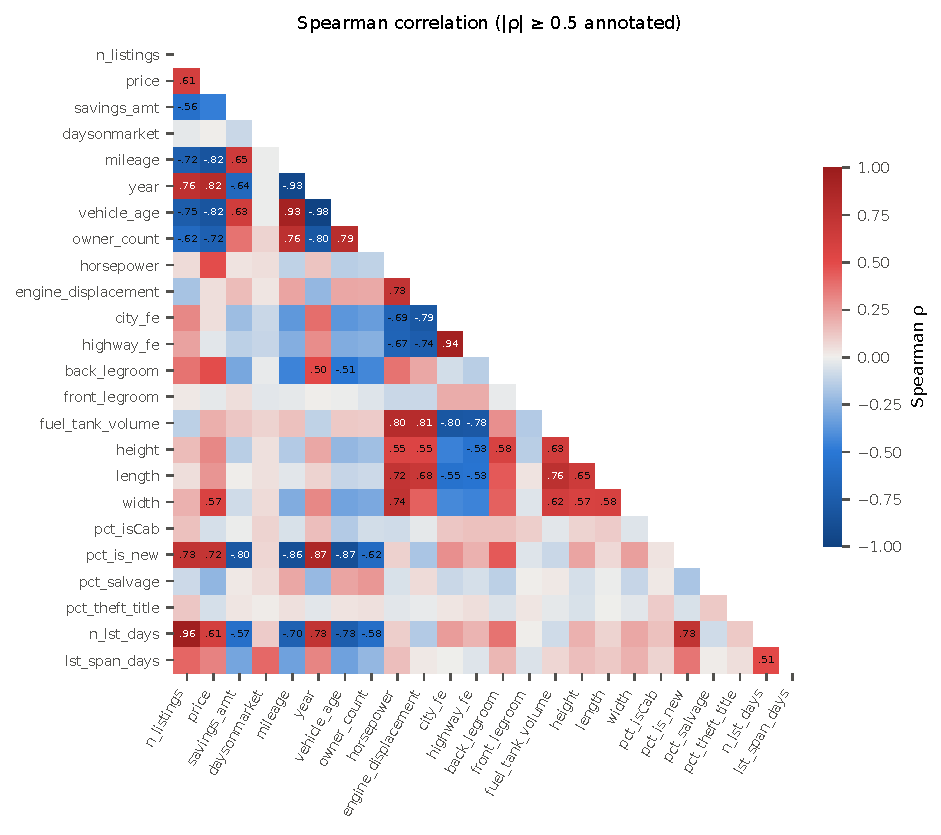
\includegraphics[width=0.80\textwidth]{m1_spearman_heatmap}
\caption{Spearman correlations of the 24 numerical attributes ($|\rho_s|\geq0.5$ annotated).}\label{fig:heat}
\end{figure*}

\begin{table}[t]
\centering
\caption{Pairs with $\max(|r|,|\rho_s|)\geq0.8$.}\label{tab:corr}
\tab{m1_corr}
\end{table}

A pair with $|\rho_s|\geq0.90$ is redundant and loses one member: \attr{year} and \attr{vehicle\_age} in favour of \attr{mileage} (continuous, least skewed wear measure), \attr{n\_listing\_days} in favour of \attr{n\_listings}, and highway in favour of city fuel economy. We also drop \attr{engine\_displacement} (missing rate; $\rho_s=0.81$ with \attr{fuel\_tank}) and \attr{new\_used\_profile} (a discretization of \attr{pct\_is\_new}). \attr{mileage} and \attr{pct\_is\_new} ($-0.86$) are both kept: they are under the threshold and describe wear and inventory mix. The criterion never looks at the target, so it cannot leak. The modelling set has \textbf{19 numerical and 5 categorical attributes}. \attr{franchise\_status} and \attr{new\_used\_profile} are almost equivalent ($V=0.90$), which is one more reason to keep only the former; the 680 sellers that break the pattern (610 used-only franchises, 70 mixed independents) remain visible through \attr{pct\_is\_new}.
